\chapter{Data Generation}
\chapterauthor{Giovanni Lucarelli}

To evaluate the performance of the proposed models under varying degrees of covariate distribution shift, we simulated a training dataset and multiple test datasets, each exhibiting a distinct degree of shift. This setup enables a comprehensive assessment of the models’ generalization capabilities.

\section{Training Data Generation}

The training dataset consists of three features, denoted as $X_1$, $X_2$, and $X_3$, and a binary target variable $Y$. The features were generated from a multivariate normal distribution $\mathcal{N}(\boldsymbol{\mu}, \boldsymbol{\Sigma})$, where each element of the mean vector $\boldsymbol{\mu}_i$ was sampled from a uniform distribution $\mathcal{U}_{[0, 1]}$, and the elements of the covariance matrix $[\boldsymbol{\Sigma}]_{i,j}$ were sampled from $\mathcal{U}_{[-1, 1]}$. To ensure the validity of the covariance matrix, after the generation, it was then transformed into a symmetric positive semi-definite matrix.
The target variable $Y$ is a binary variable with values in $\{0, 1\}$. It was generated by first constructing a second-order polynomial model with all possible interaction terms and random coefficients drawn from $\mathcal{U}_{[-1, 1]}$. The output of this polynomial was transformed using the standard logistic function to generate probabilities, which were then fed into a Bernoulli random number generator to produce the binary values of $Y$ (\cref{fig:label_dist_train}).

\begin{figure}[H]
    \centering
    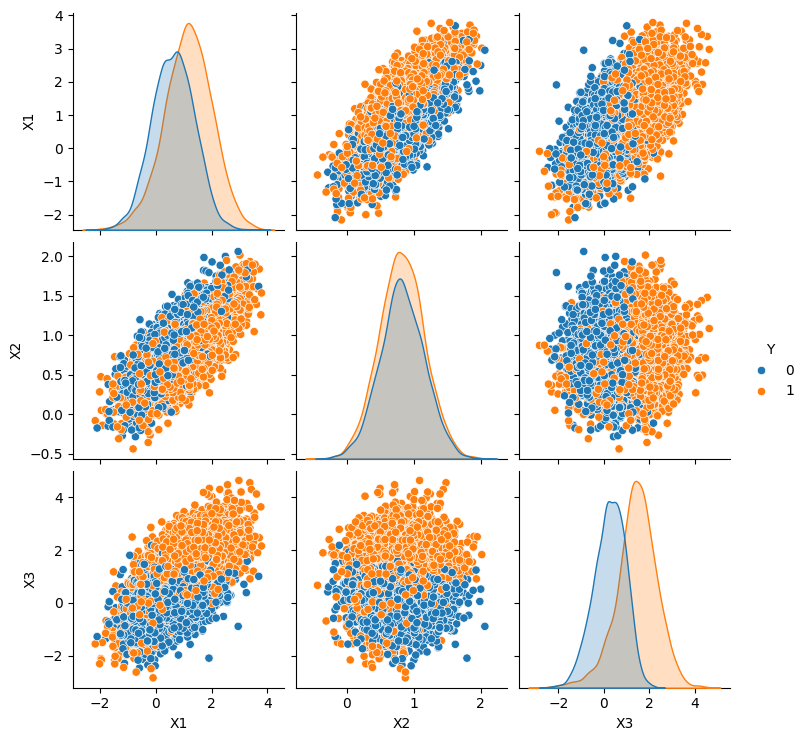
\includegraphics[width=0.7\textwidth]{assets/label_dist_train.png}
    \caption{Distribution of the target variable in the training dataset.}
    \label{fig:label_dist_train}
\end{figure}

\section{Testing Data Generation}
A fully shifted test dataset was generated from a new multivariate normal distribution $\mathcal{N}(\boldsymbol{\mu}_{0.05}, \boldsymbol{\Sigma}_s)$. Here, $\boldsymbol{\mu}_{0.05}$ represents a mean vector centered at the 5th percentile of the original $\boldsymbol{\mu}$, and $\boldsymbol{\Sigma}_s$ is a covariance matrix distinct from $\boldsymbol{\Sigma}$. This shift was deliberately designed to focus on a region of the sample space with limited representation in the training data, thereby introducing a significant covariate distribution shift. The target variable $Y$ for this dataset was generated in the same manner as in the training dataset.

\begin{figure}[H]
    \centering
    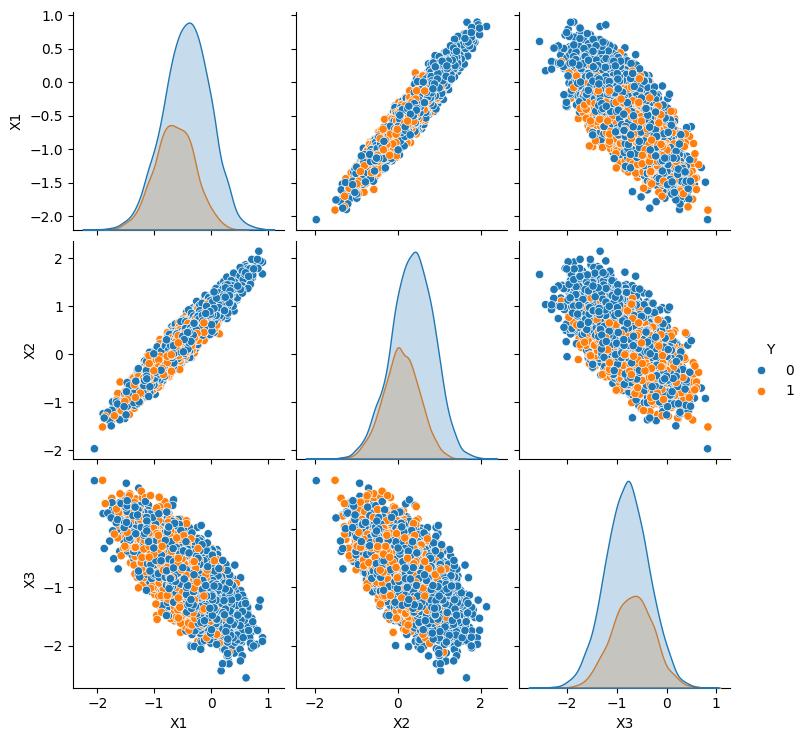
\includegraphics[width=0.7\textwidth]{assets/label_dist_fullyshift.png}
    \caption{Distribution of the target variable in the fully shifted dataset.}
    \label{fig:label_dist_fullyshift}
\end{figure}

To assess model performance across a continuum of distribution shifts, we created a series of datasets using statistical mixtures of the training dataset and the fully shifted dataset. Specifically, we defined ten datasets, $\mathcal{D}_p$, where $p \in \{0.0, 0.1, \ldots, 1.0\}$ represents the mixing probability. The dataset $\mathcal{D}_{0.0}$ corresponds to data generated from the same distribution as the training dataset (but with new samples), allowing for an evaluation of the models on unseen, unshifted data. Conversely, $\mathcal{D}_{1.0}$ corresponds to the fully shifted dataset. Intermediate values of $p$ represent datasets with increasing proportions of shifted data, enabling a systematic investigation of model robustness under various degrees of covariate distribution shift.


\begin{figure}
    \centering
    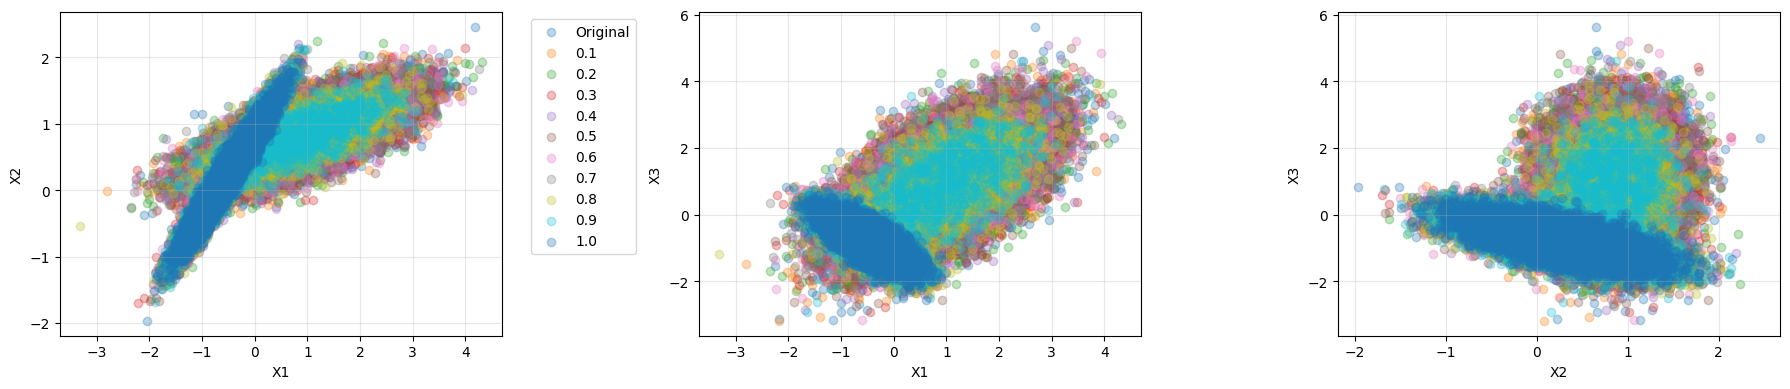
\includegraphics[width=1.0\textwidth]{assets/sparse_mix_shift.png}
    \caption{Sparseplot of the three features for all different mixing probability values of the mixtures. The full shifted dataset is the smaller one, in blue.}
    \label{fig:sparse_mix_shift}
    \vspace{1.5cm}
    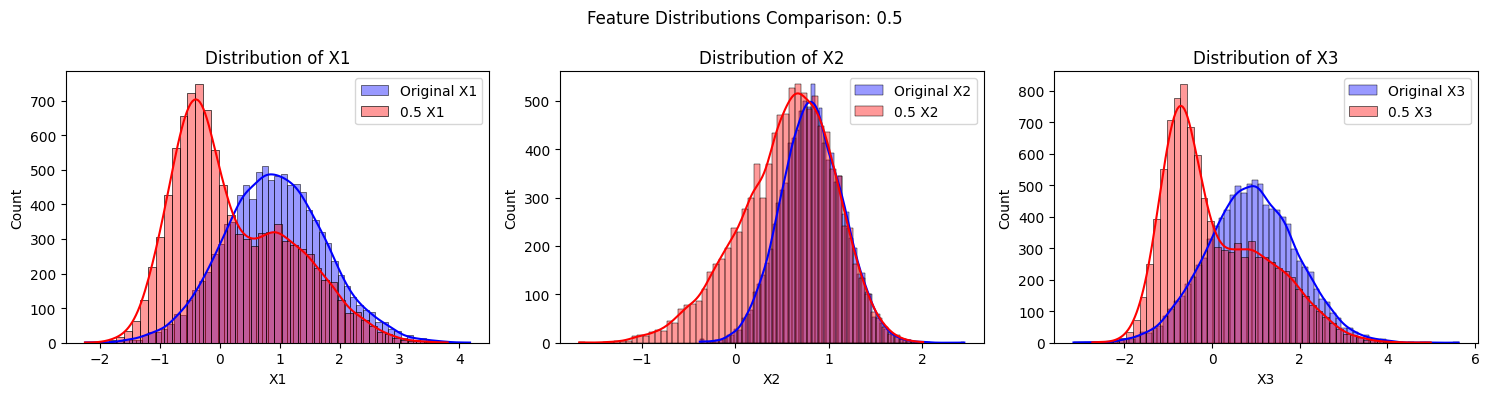
\includegraphics[width=1.0\textwidth]{assets/dist_mix05.png}
    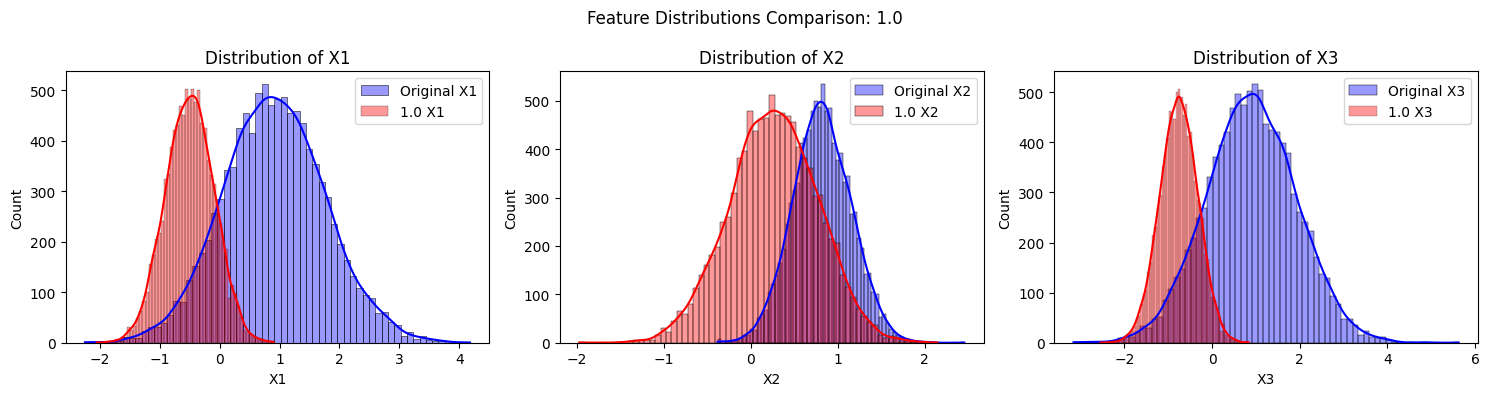
\includegraphics[width=1.0\textwidth]{assets/dist_fullshift.png}
    \caption{Comparison of feature distributions for the mixture dataset (red) and the training dataset (blue). Top: mixture with $p=0.5$. Bottom: mixture with $p=1.0$ (fully shifted dataset).}
    \label{fig:dist_mix05}
\end{figure}

As illustrated in \cref{fig:label_dist_fullyshift}, the target variable distribution in the fully shifted dataset differs substantially from that of the training dataset, exhibiting a higher proportion of instances with $Y=0$. Notably, the \textbf{imbalance ratio} (IR) of the fully shifted dataset is 2.36, compared to 1.19 in the training dataset, and this ratio increases as the mixing probability $p$ rises. It is important to take into account this variation in the distribution of the target variable when assessing the effectiveness of different models. The proposed approach is to use threshold-independent metrics such as the \textbf{ROC AUC}. This metric is particularly well-suited for evaluating model performance in the presence of class imbalance and varying decision thresholds.
